\documentclass[12pt]{article}
\usepackage[utf8]{inputenc}
\usepackage[T1]{fontenc}
\usepackage{unicode-math}
\newcommand{\EE}{\mathbb{E}}
\newcommand{\R}{\mathbb{R}}
\usepackage{amsmath,amsfonts,amssymb}
\usepackage{graphicx}
\usepackage{a4wide}
\bibliographystyle{unsrt}
\usepackage{biblatex}
\usepackage{import}
\bibliography{draft.bib}


% Comments for co-authors (optional)
\newcommand{\coauthorcomment}[2]{{\color{#1} \textbf{#2}}}

% Title and author information
% \usepackage[pagebackref=true]{hyperref}  % hyperlinks
% \renewcommand*{\backrefalt}[4]{%
%     \ifcase #1 \footnotesize{(Not cited.)}%
%     \or        \footnotesize{(Cited on page~#2)}%
%     \else      \footnotesize{(Cited on pages~#2)}%
%     \fi}
% simple URL typesetting
\usepackage{booktabs}       % professional-quality tables
\usepackage{amsfonts}       % blackboard math symbols
\usepackage{nicefrac}       % compact symbols for 1/2, etc.
\usepackage{microtype}      % microtypography
%\usepackage{slashbox,pict2e}
\usepackage{comment}
\usepackage{amssymb, amsmath, latexsym}
% \usepackage{fullpage}
\usepackage{url}

\usepackage{algorithm}
\usepackage{algorithmic}
% \usepackage{algpseudocode}


\usepackage{tabularx}
\usepackage{paralist}
\usepackage{mathtools}
%\usepackage{tcolorbox}
%\usepackage{xcolor}

\usepackage{bbm} %for indicators 1
\usepackage{wrapfig}
\usepackage{makecell}
\usepackage{multirow}
\usepackage{booktabs}

\usepackage{nicefrac}       % nice fractions

\usepackage{boxhandler}
\usepackage[flushleft]{threeparttable} % http://ctan.org/pkg/threeparttable

\usepackage{caption}
\usepackage{multirow}
\usepackage{colortbl}
\definecolor{bgcolor}{rgb}{0.8,1,1}
\definecolor{bgcolor2}{rgb}{0.8,1,0.8}
\definecolor{niceblue}{rgb}{0.0,0.19,0.56}

\usepackage{hyperref}
\hypersetup{colorlinks,linkcolor={blue},citecolor={niceblue},urlcolor={blue}}

% \usepackage{natbib}
% \bibliographystyle{abbrvnat}
% \usepackage{sidecap}
% \renewcommand{\bibname}{References}
% \renewcommand{\bibsection}{\subsubsection*{\bibname}}
%\bibliographystyle{plain}


\renewcommand{\algorithmicrequire}{\textbf{Input:}}
\renewcommand{\algorithmicensure}{\textbf{Output:}}

% \usepackage[dvipsnames]{xcolor}
\usepackage{pifont}
\definecolor{PineGreen}{RGB}{0,110,51}
\definecolor{BrickRed}{RGB}{143,20,2}
\newcommand{\cmark}{{\color{PineGreen}\ding{51}}}%
\newcommand{\xmark}{{\color{BrickRed}\ding{55}}}%


\usepackage{tikz-cd} %for a diagram

\DeclareMathOperator*{\argmax}{arg\,max}
\DeclareMathOperator*{\argmin}{arg\,min}
% \usepackage{subfigure} 
\newcommand{\Exp}{\mathbf{E}}
\newcommand{\Prob}{\mathbf{P}}
\newcommand{\R}{\mathbb{R}}
\newcommand{\eqdef}{\stackrel{\text{def}}{=}}
\newcommand{\ve}[2]{\left\langle #1 , #2 \right\rangle}
\def\<#1,#2>{\left\langle #1,#2\right\rangle}

\newcommand{\oldstuff}[1]{ {\small \color{blue} #1}}
\newcommand{\redstuff}[1]{ {\small \color{red} #1}}

% for even table widths
\newcolumntype{Y}{>{\centering\arraybackslash}X}


\usepackage{xspace}

% Define the figure size
\newcommand\figscale{0.25}
\newcommand\evofigscale{0.21}


%\newcommand{\squeeze}{\textstyle} % when deployed
\newcommand{\squeeze}{} % when not deployed

\newcommand{\algname}[1]{{\sf  #1}\xspace}
\newcommand{\algnamex}[1]{{\sf #1}\xspace}

\newcommand\tagthis{\addtocounter{equation}{1}\tag{\theequation}}

\newcommand{\circledOne}{\text{\ding{172}}}
\newcommand{\circledTwo}{\text{\ding{173}}}
\newcommand{\circledThree}{\text{\ding{174}}}
\newcommand{\circledFour}{\text{\ding{175}}}
\newcommand{\circledFive}{\text{\ding{176}}}
\newcommand{\circledSix}{\text{\ding{177}}}
\newcommand{\circledSeven}{\text{\ding{178}}}
\newcommand{\circledEight}{\text{\ding{179}}}
\newcommand{\circledNine}{\text{\ding{180}}}
\newcommand{\circledTen}{\text{\ding{181}}}
\newcommand{\qed}{\hfill\blacksquare}
% TO DO NOTES 
\usepackage[colorinlistoftodos,bordercolor=orange,backgroundcolor=orange!20,linecolor=orange,textsize=scriptsize]{todonotes}

\newcommand{\alexander}[1]{\todo[inline]{{\textbf{Alexander:} \emph{#1}}}}
\newcommand{\eduard}[1]{\todo[inline]{{\textbf{Eduard:} \emph{#1}}}}
\newcommand{\nikita}[1]{\todo[inline]{{\textbf{Nikita:} \emph{#1}}}}
\newcommand{\Aleksandr}[1]{\todo[inline]{{\textbf{Aleksandr:} \emph{#1}}}}



\renewcommand{\Re}{\mathrm{Re}}
\renewcommand{\Im}{\mathrm{Im}}
\newcommand{\Sp}{\mathrm{Sp}}
\newcommand{\Id}{\mathrm{Id}}

\newcommand{\Tr}{\mathrm{Tr}}
\newcommand{\KL}{\mathrm{KL}}

% caligraphic
\newcommand{\cA}{{\cal A}}
\newcommand{\cB}{{\cal B}}
\newcommand{\cC}{{\cal C}}
\newcommand{\cD}{{\cal D}}
\newcommand{\cE}{{\cal E}}
\newcommand{\cF}{{\cal F}}
\newcommand{\cG}{{\cal G}}
\newcommand{\cH}{{\cal H}}
\newcommand{\cJ}{{\cal J}}
\newcommand{\cK}{{\cal K}}
\newcommand{\cL}{{\cal L}}
\newcommand{\cM}{{\cal M}}
\newcommand{\cN}{{\cal N}}
\newcommand{\cO}{{\cal O}}
\newcommand{\cP}{{\cal P}}
\newcommand{\cQ}{{\cal Q}}
\newcommand{\cR}{{\cal R}}
\newcommand{\cS}{{\cal S}}
\newcommand{\cT}{{\cal T}}
\newcommand{\cU}{{\cal U}}
\newcommand{\cV}{{\cal V}}
\newcommand{\cX}{{\cal X}}
\newcommand{\cY}{{\cal Y}}
\newcommand{\cW}{{\cal W}}
\newcommand{\cZ}{{\cal Z}}
\newcommand{\Var}{\mathrm{Var}}

% matrices
\newcommand{\mA}{{\bf A}}
\newcommand{\mB}{{\bf B}}
\newcommand{\mC}{{\bf C}}
\newcommand{\mE}{{\bf E}}
\newcommand{\mF}{{\bf F}}
\newcommand{\mG}{{\bf G}}
\newcommand{\mH}{{\bf H}}
\newcommand{\mI}{{\bf I}}
\newcommand{\mJ}{{\bf J}}
\newcommand{\mK}{{\bf K}}
\newcommand{\mL}{{\bf L}}
\newcommand{\mM}{{\bf M}}
\newcommand{\mN}{{\bf N}}
\newcommand{\mO}{{\bf O}}
\newcommand{\mP}{{\bf P}}
\newcommand{\mQ}{{\bf Q}}
\newcommand{\mR}{{\bf R}}
\newcommand{\mS}{{\bf S}}
\newcommand{\mT}{{\bf T}}
\newcommand{\mU}{{\bf U}}
\newcommand{\mV}{{\bf V}}
\newcommand{\mW}{{\bf W}}
\newcommand{\mX}{{\bf X}}
\newcommand{\mY}{{\bf Y}}
\newcommand{\mZ}{{\bf Z}}

\newcommand{\sign}{\mathrm{sign}}
\newcommand{\cnorm}{x}
\newcommand{\EE}{\mathbb{E}}
\newcommand{\PP}{\mathbb{P}}
\newcommand{\CC}{\mathbb{C}}
\newcommand{\VV}{\mathbf{V}}

\newcommand{\prox}{\mathop{\mathrm{prox}}\nolimits}


\newcommand{\proxR}{\prox_{\gamma R}}
\newcommand{\proxkR}{\prox_{\gamma^k R}}
\newcommand{\mean}{\overline}
\newcommand{\sumin}{\sum_{i=1}^n}

\newcommand{\tx}{\widetilde{x}}
\newcommand{\tX}{\widetilde{X}}
\newcommand{\ty}{\widetilde{y}}
\newcommand{\tF}{\widetilde{F}}

\newcommand{\tnabla}{\widetilde{\nabla}}


\newcommand{\hx}{\widehat{x}}
\newcommand{\hy}{\widehat{y}}


\def\Bxi{\boldsymbol{\xi}}

\def\clip{\texttt{clip}}
\def\avg{\texttt{avg}}
\def\gap{\texttt{Gap}}



\usepackage{hyperref}
\graphicspath{{plots/}}

\usepackage{makecell}

\usepackage{accents}
\newlength{\dhatheight}
\newcommand{\doublehat}[1]{%
    \settoheight{\dhatheight}{\ensuremath{\hat{#1}}}%
    \addtolength{\dhatheight}{-0.35ex}%
    \hat{\vphantom{\rule{1pt}{\dhatheight}}%
    \smash{\hat{#1}}}}


\usepackage{pgfplotstable} % loads pgfplots which loads tikz
\usetikzlibrary{automata, positioning, arrows, shapes, fit, calc, intersections}
\usepgfplotslibrary{statistics}

\newcommand{\dotprod}[2]{\langle #1,#2 \rangle} % Скалярное произведение




\def\la{\langle}
\def\ra{\rangle}
\usepackage{enumitem}
\usepackage{algorithm}
\usepackage{algorithmic}
\usepackage{algpseudocode}
\usepackage{subcaption}
\usepackage{graphicx}
\usepackage{amsthm}
\newtheorem{assumption}{Assumption}
\newtheorem{lemma}{Lemma}
\newtheorem{proposition}{Proposition}
\newtheorem{theorem}{Theorem}
\newtheorem{corollary
}{Corollary
}
\newtheorem{definition}{Definition}
\newtheorem{remark}{Remark}

\title{Sign operator for $(L_0, L_1)$-smooth optimization}

\author{
  Mark Ikonnikov\\
  \texttt{ikonnikov.mi@phystech.edu}
  \and
  Nikita Kornilov\\
  \texttt{kornilov.nm@phystech.edu}
}

\date{\today}

\begin{document}
\maketitle

\begin{abstract}
In Machine Learning, the non-smoothness of optimization problems, the high cost of communicating gradients between workers, and severely corrupted data during training necessitate generalized optimization approaches. This paper explores the efficacy of sign-based methods~\cite{pmlr-v80-bernstein18a}, which address slow transmission by communicating only the sign of each minibatch stochastic gradient. We investigate these methods within $(L_0, L_1)$-smooth problems~\cite{gorbunov}, which encompass a wider range of problems than the $L$-smoothness assumption. Furthermore, under the assumptions above, we investigate techniques to handle heavy-tailed noise~\cite{Kornilov2025}, defined as noise with bounded $\kappa$-th moment $\kappa \in (1,2]$. This includes the use of SignSGD with Majority Voting in the case of symmetric noise. We then attempt to extend the findings to convex cases using error feedback~\cite{karimireddy}.
\end{abstract}

\paragraph{Keywords:} Sign-based methods, $(L_0, L_1)$-smoothness, high-probability convergence, heavy-tailed noise.

\paragraph{ Highlights below to be fixed later (these are our hopes for the paper)}

\paragraph{ Highlights:}
\begin{enumerate}
\item Proves convergence of sign-based methods for $(L_0, L_1)$-smooth optimization
\item Handles heavy-tailed noise with high-probability convergence guarantees
\item Extends sign-based optimization to convex functions using error feedback
\end{enumerate}

\section{Introduction}


\import{./}{intro}


\section{Computational experiment}

\section*{THIS PART WILL BE DELETED}

\begin{figure}[!h]
    \centering
    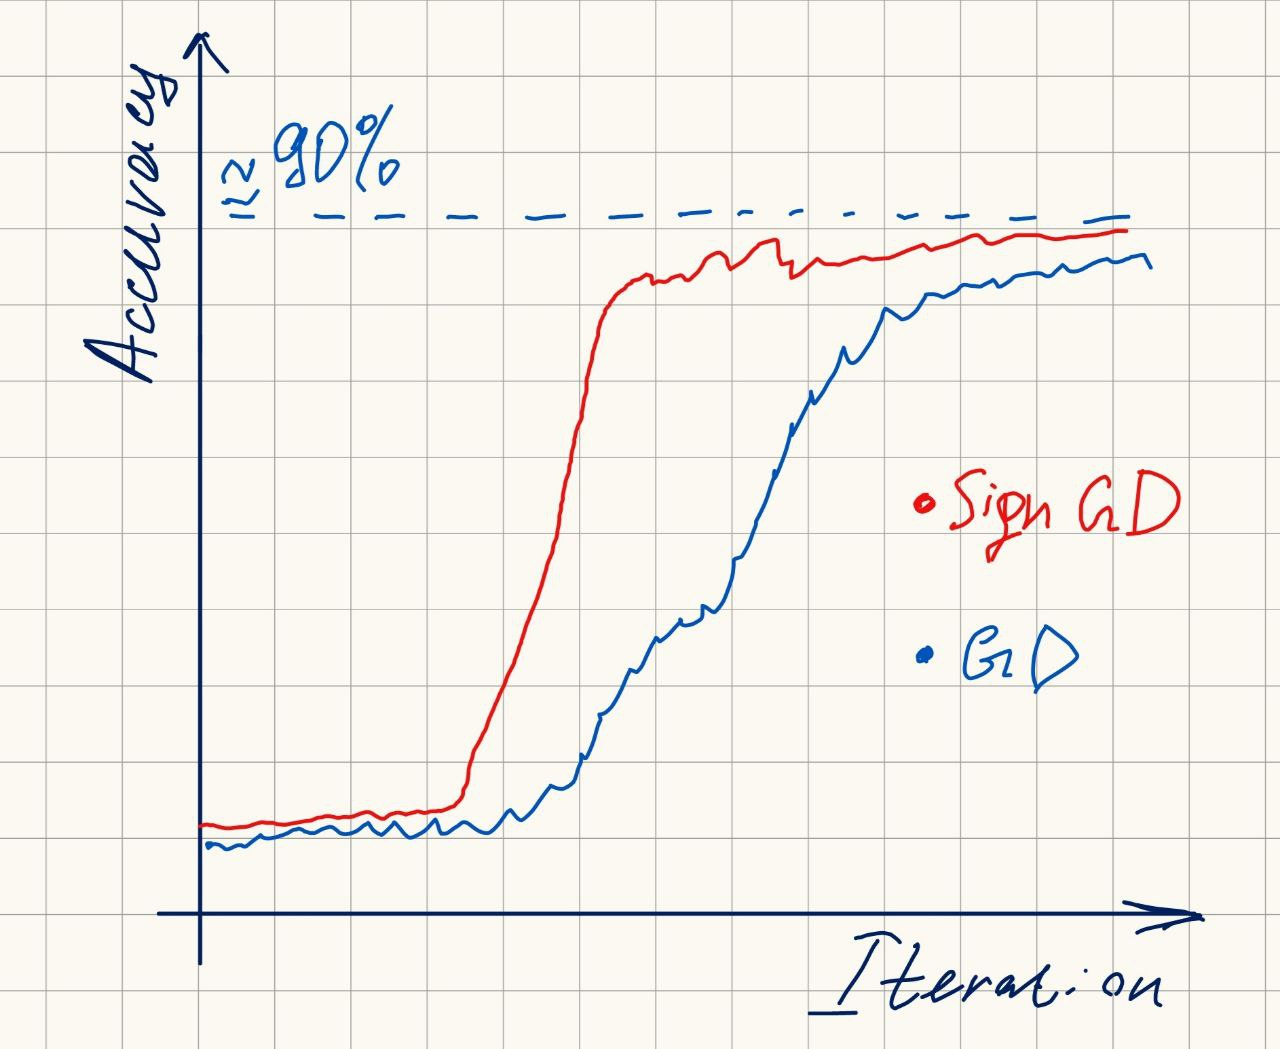
\includegraphics[width=0.3\textwidth]{drawing.jpg}
    \caption{Performance of GD, SignGD}
    \label{fig:logreg}
\end{figure}

The computational experiment aims to compare the performance of standard gradient descent (GD) and sign-based gradient descent (Sign-GD) in training a logistic regression model, highlighting the advantages of sign-based methods under L0 and L1 smoothness assumptions. Performance will be evaluated based on accuracy and iteration number, with minimal tuning to emphasize simplicity.

The experiment compares standard gradient descent (GD) and sign-based gradient descent (Sign-GD) on an open-source binary classification dataset "Mushrooms". Below is a mini-report based on expected outcomes.
The preliminary plot (hand-drawn) shows Sign-GD achieving comparable or better performance with faster convergence, consistent with $(L_0, L_1)$ smoothness assumptions.

Comments: 
The idea is based on the fact that logistic regression function $l(z,y) = \ln (1 + \exp(-yz)$  is both smooth and $(L_0, L_1)$-smooth, with $L = || y ||^2$ and $L_0 = 0, L_1 = || y ||$ which can be much smaller than $L$. Sign-GD slightly outperforms GD in accuracy and convergence time, suggesting that the sign-based update leverages smoothness assumptions effectively. The simplicity of the approach (no complex tuning) aligns with the minimal-effort goal. These results do not contradict the experiment’s aim to showcase sign-based method advantages.
\begin{figure}[!h]
    \centering
    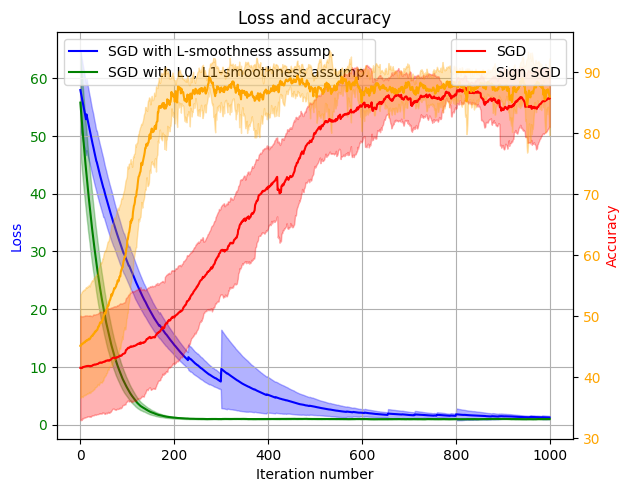
\includegraphics[width=0.9\textwidth]{basic_experiment2.png}
    \caption{Logistic regression on Mushroom Dataset.\newline Performance of GD, SignGD with $L_1 $-tuned step size}
    \label{fig:logreg}
\end{figure}


\newpage


\section{Theory}

In this section, we present our novel convergence guarantees with high probability for existing sign-based methods for non-convex functions with heavy-tailed noise in gradient estimates. For each algorithm, we provide an explicit optimal tuning for the parameters. If function's smoothness constant and noise's characteristics are not given, we state the rates for arbitrary tuning. All proofs are located in Appendix \ref{app: proofs}.

\subsection{Assumptions}
 
\begin{assumption}[Lower bound]\label{as: bounded}
    The objective function $f$ is lower bounded by $f^* > -\infty$, i.e., $f(x) \geq f^*, \forall x \in \R^d.$
\end{assumption}
\begin{assumption}[$(L_0, L_1)$-Smoothness]\label{as: smooth}
    The objective function $f$ is differentiable and $(L_0, L_1)$-smooth, i.e., for the positive constants $(L_0, L_1)$
    $$
\|\nabla f(x) - \nabla f(y)\| \leq \left(L_0 + L_1  \|\nabla f(u)\|\right) \|x - y\|,
\quad \forall x, y \in \R^d. $$
\end{assumption}
\begin{assumption}[Heavy-tailed noise in gradient estimates]\label{as: pBCM}
    The unbiased estimate $\nabla f (x, \xi)$  has bounded $\kappa$-th moment $\kappa \in (1,2]$ for each coordinate, i.e., $\forall x \in \R^d$: 
    \begin{itemize}
        \item $\EE_\xi [\nabla f (x, \xi)] = \nabla f(x),$
        \item $\EE_\xi [|\nabla f (x, \xi)_i - \nabla f(x)_i|^\kappa] \leq \sigma_i^\kappa, i \in \overline{1,d},$
    \end{itemize}
    where $\Vec{\sigma} = [\sigma_1, \dots, \sigma_d]$ are non-negative constants.
    If $\kappa = 2$, then the noise is called a bounded variance. 
\end{assumption}


\subsection{\algname{SignSGD} and its HP convergence properties} 
We begin our analysis with the simplest of sign-based methods, namely \algname{SignSGD} (Alg. \ref{alg: signSGD}) and prove a general lemma on its convergence with high probability.
\begin{algorithm}[ht!]
\caption{\algname{SignSGD} }
\label{alg: signSGD}   
\begin{algorithmic}[1]
\Require
Starting point $x^1 \in \R^d$, number of iterations $T$, stepsizes  $\{\gamma_k\}_{k=1}^{T}$.
\For{$k=1,\ldots, T$}
    \State Sample $\xi^k$ and compute estimate $g^k =     \nabla f(x^k, \xi^k)$;
    \State Set $x^{k+1} = x^k - \gamma_k \cdot     \sign(g^k)$;
\EndFor
\Ensure
uniformly random point from $\{x^1, \dots, x^T\}$ . 
\end{algorithmic}
\end{algorithm}

 In order to achieve accuracy $\varepsilon$, the noise $\|\Vec{\sigma}\|_1$ have not to exceed $\varepsilon$.  The first way to lower the noise is to use batching. 
\subsection{\algname{SignSGD} with batching}\label{sec:minibatch sign sgd}

\begin{algorithm}[ht!]
\caption{\algname{minibatch-SignSGD} }
\label{alg:minibatch-signSGD}   
\begin{algorithmic}[1]
\Require Starting point $x^1 \in \R^d$, number of iterations $T$, stepsizes  $\{\gamma_k\}_{k=1}^{T}$, batchsizes $\{B_k\}_{k=1}^{T}$.

\For{$k=1,\ldots, T$}
\State Sample $\{\xi^k_i\}_{i=1}^{B_k}$
\State Compute gradient estimate  $g^k = \sum_{i=1}^{B_k} \nicefrac{\nabla f(x^k, \xi^k_i)}{B_k}$;
\State Set $x^{k+1} = x^k - \gamma_k \cdot \sign(g^k)$;
\EndFor
\Ensure uniformly random point from $\{x^1, \dots, x^{T}\}$ . 
\end{algorithmic}
\end{algorithm}

\section{$(L_0, L_1)$ smoothness}
\begin{lemma}(Symmetric  $(L_0, L_1)$-smoothness) \label{lem: L_0,L_1 smoothness}
    Function $f:\R^d \to \R$ is asymmetrically $(L_0, L_1)$-smooth, i.e., for all $x,y \in \R^d$, it holds
    \begin{equation}
        \|\nabla f(x) - \nabla f(y)\|_2 \leq (L_0 + L_1\|\nabla f(y)\|_2)\exp(L_1\|x-y\|_2)\|x-y\|_2.
    \end{equation}
    Moreover, it implies
    \begin{eqnarray}
        f(y) \leq f(x) + \la \nabla f(x), y -x \ra + \frac{L_0 + L_1\|\nabla f(x)\|_2 }{2}\exp(L_1\|x-y\|_2)\|x-y\|_2^2.
    \end{eqnarray}
\end{lemma}
\subsection{Proof of $(L_0,L_1)$ \algname{SignSGD} General Convergence }  
\begin{proof}
    Consider the $k$-th step of \algname{SignSGD}. We use $(L_0, L_1)$ smoothness of function $f$ (Lemma \ref{lem: L_0,L_1 smoothness}) to estimate:
    \begin{eqnarray}
        f(x^{k+1}) - f(x^k) &\leq& \la \nabla f (x^k), x^{k+1} - x^k \ra + \frac{L_0 + L_1\|\nabla f(x^k)\|_2 }{2}\exp(L_1\|x^{k+1} - x^k\|_2)\|x^{k+1} - x^k\|_2^2 \notag \\
        &=& - \gamma_k  \frac{\la \nabla f (x^k), \sign(g^k) \ra}{\|\nabla f (x^k)\|_1} \cdot \|\nabla f (x^k)\|_1 + \frac{L_0d \gamma_k^2}{2}\exp(L_1\sqrt{d}\gamma_k) \notag \\ &+& \frac{ L_1d\gamma_k\exp(L_1\sqrt{d}\gamma_k) }{2}\cdot \gamma_k \|\nabla f(x^k)\|_2 \notag \\
         &=& - \gamma_k  \frac{\la \nabla f (x^k), \sign(g^k) \ra}{\|\nabla f (x^k)\|_1} \cdot \|\nabla f (x^k)\|_1 + \frac{L_0d \gamma_k^2}{2}\exp(L_1\sqrt{d}\gamma_k) \notag \\ &+&  \frac{ L_1\sqrt{d}\gamma_k\exp(L_1\sqrt{d}\gamma_k) }{2}\cdot \gamma_k \|\nabla f(x^k)\|_1.\notag
    \end{eqnarray}
    Consequently, after summing all $T$ steps, we obtain the next equation.
    We introduce the following terms  $\phi_k := \frac{\la \nabla f (x^k), \sign(g^k) \ra}{\|\nabla f (x^k)\|_1} \in [-1,1]$, $\psi_k := \EE[\phi_k| x^{k }]$ and $D_k := - \gamma_k (\phi_k - \psi_k)\|\nabla f (x^k)\|_1$. We note that $D_k$ is a martingale difference sequence ($\EE[D_k|D_{k-1}, \dots, D_k] = 0$) and satisfies 
    $$\exp\left( \frac{D_k^2}{4\gamma_k^2\|\nabla f (x^k)\|_1^2}\right) = \exp \left(\frac{(\phi_k - \psi_k)^2}{4}\right) \leq e.$$
    Applying Measure Concentration Lemma to MSD  we derive the bound for all $\lambda > 0$ with probability at least $1 - \delta$.
     We then use norm relation and $(L_0,L_1)$-smoothness to estimate maximum gradient norm for all $k \in \overline{2,T+1}:$
    \begin{eqnarray}
        \|\nabla f (x^k)\|_1/\sqrt{d} &\leq& \|\nabla f (x^k)\|_2 \leq \|\nabla f (x^k) - \nabla f (x^{k-1}) + \nabla f (x^{k-1}) \|_2  \notag \\
    &\leq& \|\nabla f (x^k) - \nabla f (x^{k-1})\|_2 +  \|\nabla f (x^{k-1}) \|_2 \notag \\
    &\leq&  (L_0 + L_1\|\nabla f(x^{k-1})\|_2)\exp(L_1\|x^{k} - x^{k-1}\|_2)\|x^{k} - x^{k-1}\|_2 + \|\nabla f (x^{k-1})\|_2  \notag\\
    &\leq&  (L_0 + L_1\|\nabla f(x^{k-1})\|_2)\exp(L_1\sqrt{d}\gamma_k )\sqrt{d}\gamma_k + \|\nabla f (x^{k-1})\|_2.  \notag
    \end{eqnarray}
    At this point, we take $\gamma_k \leq \frac{1}{48L_1d\log\frac1\delta \sqrt{d}}$ to obtain
    \begin{eqnarray}
        \|\nabla f (x^k)\|_1/\sqrt{d} &\leq& 2L_0\sqrt{d}\gamma_k  + \frac{\|\nabla f (x^{k-1})\|_2}{48d \log \frac1\delta}+ \|\nabla f (x^{k-1})\|_2 \notag \\
    &\leq&   2L_0\sqrt{d}\sum_{\tau=1}^{k-1}\gamma_\tau + \sum_{\tau=1}^{k-1}\frac{\|\nabla f (x^{\tau})\|_2}{48d \log \frac1\delta} + \|\nabla f (x^1)\|_2 \notag \\
    &\leq&   2L_0\sqrt{d}\sum_{\tau=1}^{k-1}\gamma_\tau + \sum_{\tau=1}^{k-1}\frac{\|\nabla f (x^{\tau})\|_1}{48d \log \frac1\delta} + \|\nabla f (x^1)\|_1. \notag
    \end{eqnarray}
    Hence, the choice of $\lambda$ yields with probability at least $1 - \delta$:

    Next, we estimate each term $\psi_k \|\nabla f (x^k)\|_1$ in the previous sum:
\begin{eqnarray}
\psi_k \|\nabla f (x^k)\|_1 &=& \EE \left[ \la \nabla f (x^k), \sign(g^k) \ra| x^k \right] \notag \\
&=& \|\nabla f (x^k)\|_1 - \sum_{i=1}^d 2 |\nabla f (x^k)|_i \cdot \mathbb{P}(\sign(\nabla f (x^k))_i\neq \sign(g^k)_i | x^k).\label{eq: line with prob sign}
\end{eqnarray}
For each coordinate, we have a bound derived from Markov's inequality   followed by Jensen’s inequality:
\begin{eqnarray}
    \mathbb{P}(\sign(\nabla f (x^k))_i \neq \sign(g^k)_i | x^k) &\leq& \mathbb{P}(|\nabla f (x^k)_i -  g^k_i| \geq |\nabla f (x^k)_i| |  x^k)  
    \leq \frac{\EE_{\xi^k}[|\nabla f (x^k)_i - g^k_i| ]}{|\nabla f (x^k)_i|} \notag \\ &\leq& \frac{(\EE_{\xi^k}[|\nabla f (x^k)_i - g^k_i|^\kappa ])^\frac{1}{\kappa}}{|\nabla f (x^k)_i|}  \leq \frac{\sigma_i }{|\nabla f (x^k)_i|}. \label{eq:Prob sign not eq simple}
\end{eqnarray}
Hence, the whole sum can be bounded as 
\begin{eqnarray}
    \sum_{i=1}^d 2 |\nabla f (x^k)|_i \cdot \mathbb{P}(\sign(\nabla f (x^k))_i\neq \sign(g^k)_i | x^k)
    &\leq& 2 \|\Vec{\sigma}\|_1. \notag \notag 
\end{eqnarray}
Finally, we put this bound in telescopic sum and obtain our bound.
Plug in constant stepsizes $\gamma_k \equiv \gamma \leq \frac{1}{48L_1d\log\frac1\delta \sqrt{d}}$.

\textbf{Optimal tuning.} In case $\varepsilon \geq  \frac{8L_0}{L_1\sqrt{d}}$, we use stepsize $\gamma = \frac{1}{48L_1d\log\frac1\delta \sqrt{d}} \Rightarrow 80 L_0 d\gamma \log(\nicefrac{1}{\delta}) \leq \varepsilon/2$ and  batchsize $8\frac{\|\Vec{\sigma}\|_1}{B^{\frac{\kappa-1}{\kappa}}} \leq \varepsilon/2 \Rightarrow B_k \equiv \max \left\{1,  \left(\frac{16\|\Vec{\sigma}\|_1}{\varepsilon}\right)^\frac{\kappa}{\kappa-1}\right\}$. The number of iterations  $T$ is chosen to bound the first term: $T = O\left(\frac{\Delta_1 L_1  \log \frac1\delta d^\frac{3}{2}}{\varepsilon}\right).$ The total number of oracle calls is:
\begin{eqnarray}
    \varepsilon &\geq&   \frac{8L_0}{L_1\sqrt{d}} \quad \Rightarrow \quad N = O\left(\frac{\Delta_1 L_1  \log(\nicefrac{1}{\delta} ) d^\frac{3}{2}}{\varepsilon}\left[1 +  \left(\frac{\|\Vec{\sigma}\|_1}{\varepsilon}\right)^\frac{\kappa}{\kappa-1}\right]\right), \notag \\
\varepsilon &<& \frac{8L_0}{L_1\sqrt{d}} \quad \Rightarrow \quad N = O\left(\frac{\Delta_1L_0\log(\nicefrac{1}{\delta} ) d }{\varepsilon^2}\left[1 +  \left(\frac{\|\Vec{\sigma}\|_1}{\varepsilon}\right)^\frac{\kappa}{\kappa-1}\right]\right). 
\end{eqnarray}
\end{proof}





\printbibliography

\end{document}